%!TeX root=../tese.tex
%(dica para o editor de texto: este arquivo é parte de um documento maior)
% para saber mais: https://tex.stackexchange.com/q/78101/183146

\chapter{Redes neurais artificiais}
\label{cap:redes}

Neste capítulo são apresentados alguns conceitos básicos de \defi{aprendizado de máquina}, com foco nos algoritmos de redes neurais artificiais, em especial o \defi{perceptron}, cujo desenvolvimento foi inspirado nas redes neurais biológicas, ou seja, os neurônios e suas conexões no cérebro, conforme descrito por Kopec \citep{classic}.

Pode-se classificar as técnicas de aprendizado de várias formas, de acordo com alguma de suas características. Por exemplo, Géron \citep{hands} utiliza o grau de supervisão humana durante o seu funcionamento para classificá-los em aprendizado supervisionado ou não-supervisionado. Isto quer dizer que durante o treinamento são fornecidos um conjunto de consultas e de respostas esperadas. Tais respostas foram dadas por humanos, daí o termo `supervisão humana'.

\section{Aprendizado de máquina supervisionado}

 Um algoritmo de \defi{aprendizado supervisionado} é usado quando conhecemos os rótulos dos dados que estamos utilizando. De modo geral já temos de antemão as respostas às consultas para os dados utilizados no treinamento. Por exemplo, se estamos classificando fotos de animais, possuímos um conjunto de fotos em que já sabemos quais são de gatos, cachorros, etc.

 O ato de rotular previamente os dados que usamos no treinamento é o que designamos de supervisão humana. Uma vez \emph{treinado}, o algoritmo recebe uma foto, ou seja, uma nova consulta e então fornece a resposta se essa é a foto de um gato, ou cachorro, ou qualquer outra resposta daquelas que foram dadas como exemplos durante o treinamento.

Dentro do aprendizado supervisionado temos duas técnicas principais. A regressão é usada para prever valores, ou seja, fornecer dados do futuro, e a classificação é usada para prever os rótulos dos dados, que também são chamados de classes. Neste texto os termos ``algoritmo'' e ``técnica'' serão usados livremente como sinônimos, pois uma técnica de aprendizado de máquina, no contexto atual, é obviamente um algoritmo executado no computador.

Colocar exemplos...

\section{Aprendizado não-supervisionado}

Nesse tipo de aprendizado de máquina, não sabemos os rótulos dos dados que estamos lidando, assim o algoritmo poderá agrupar os dados de forma automática, por exemplo, se estivermos lidando com problemas de classificação. Aqui, as consultas podem ser coisas como ``quantos são os perfis dos clientes'' ou ``quantas espécies de flores existem nestas fotos'', e assim por diante.

Alguns métodos não-supervisionados de aprendizado foram enumeradas por Géron \citep{hands}. O \textbf{agrupamento} de dados similares sob uma inspiração geométrica. Nesse caso os dados são agrupados conforme suas posições num determinado espaço e utiliza-se algoritmos como $k$-vizinhos, $k$-means, $k$-medians, etc. Exemplos de aplicações são agrupamento de produtos em supermercados, interesses comuns de clientes em sites de conteúdo digital, etc.

Outra técnica é a \textbf{detecção de anomalias}, cujo objetivo é ter uma descrição de como os dados considerados ``normais'' se parecem, e usa-se esse agrupamento para detectar se novos dados estariam ``fora'' desse padrão. Um exemplo é a detecção de fraudes.

Também pode-se citar sobre a técnica de \textbf{estimação de densidades}, que tem como objetivo a estimação da função densidade de probabilidade de um conjunto de dados gerados por algum processo aleatório.

Colocar exemplos...

\section{Técnicas de classificação}

É uma das técnicas principais do aprendizado supervisionado, problemas desse tipo buscam aprender com um conjunto de dados previamente rotulados. Consultas do tipo ``a qual grupo pertence este cliente'' ou ``que animal há nesta foto'' podem ser modeladas por esses algoritmos. De modo geral, ele responde a consultas que dizem respeito às classes dos dados, e atribui para novos dados alguma classe que pertence ao conjunto de classes que usamos para rotular os dados iniciais.

Existem vários tipos de algoritmos de classificação, dentre eles podemos mencionar: máquina de vetor suporte (\eng{support vector machine}, SVM), árvores de decisão, florestas aleatórias que são um conjunto de muitas de árvores de decisão aleatoriamente definidas e, finalmente, as redes neurais artificiais.

Todas essas técnicas podem ser usadas para classificação linear ou não-linear, no sentido em que valores eles estão classificando, assim como na forma que está sendo feita essa classificação. Se visualizarmos os dados num espaço bidimensional, um algoritmo de classificação linear irá separar as classes de dados por retas, enquanto que um classificador não-linear poderá usar outra curva qualquer para a separação. 

Abstraindo o espaço bidimensional para os espaços multidimensionais dos dados que são comumente analisados, podemos pensar em hiperplanos, estruturas ($n{-}1$-dimensionais de espaços $n$-dimensionais, para o caso dos classificadores lineares, ou subespaços quaisquer para os não-lineares.

Colocar exemplos de aplicações...

\section{A rede neural perceptron}

Uma rede neural artificial é um dentre vários métodos de classificação, ou seja, de aprendizado supervisionado. De acordo com Kopec \citep{classic}, ele é utilizado como um classificador não-linear, e por isso pode ser utilizado para classificar ou prever quaisquer tipos de dados ou funções, que podem ou não ter uma relação linear com o tempo ou com qualquer outro domínio no qual estejam definidos.

Uma definição para uma rede neural artificial dada por Rosangela Ballini \citep{doutorado} é a de um sistema de processamento paralelo e distribuído baseado no sistema nervoso biológico, sendo compostos por elementos computacionais chamados neurônios, arranjados em padrões semelhantes às redes biológicas.

Na figura~\ref{fig:neuron} está uma representação de um neurônio biológico. Ele recebe impulsos elétricos de entrada através dos dentritos, que são transmitidos ou não através do núcleo, caso sejam ativados por ele, para os terminais de saída dos axônios. Os neurônios se comunicam através de sinapses, que são ligações entre os dentritos de um e os axônios de outro que realizam a transmissão dos sinais. 

\begin{figure}[htb]
\centering
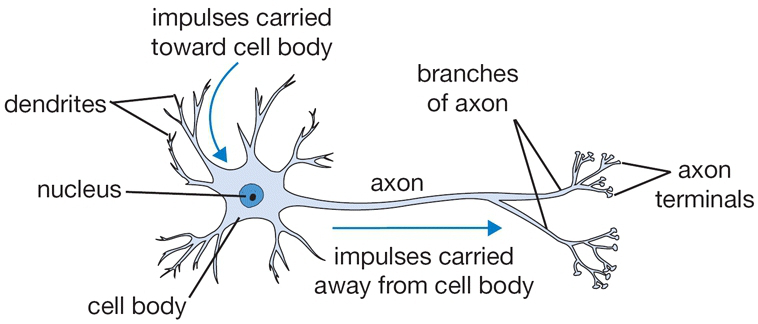
\includegraphics[width=8cm]{figuras/neuron}
\caption{Representação de um neurônio biológico.\footnote{Extraído de \url{https://cs231n.github.io/neural-networks-1/}}}
\label{fig:neuron}
\end{figure}

Dá-se o nome de \eng{perceptron} de camada única (\eng{single-layer perceptron}) ou simplesmente \eng{perceptron} a uma das primeiras e mais simples rede neural artificial a ser criada. Uma ilustração conceitual dela está na figura~\ref{fig:perceptron}. Mais recentemente foram criadas várias outras versões dessa rede, dentre as quais podemos citar o \eng{perceptron} de multi-camadas (\eng{multi-layer perceptron}). 

\begin{figure}[htb]
\centering
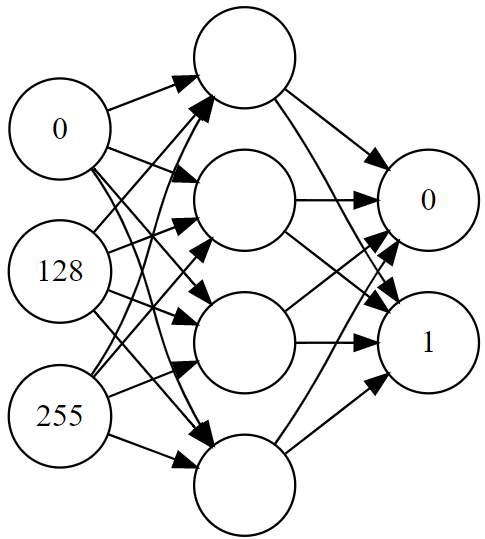
\includegraphics[width=6cm]{figuras/perceptron}
\caption{Rede neural simples, o perceptron de camada única.}
\label{fig:perceptron}
\end{figure}

Os neurônios são representados por círculos, dentro deles há um valor numérico que intuitivamente podemos atribuir ao nível ou grau de ativação do neurônio, mesmo que no caso biológico se restrinja aos valores $0$ e $1$, ou seja, ativados ou não. Cada coluna de neurônios representa uma camada, nesse caso, da esquerda para a direita temos a camada de entrada, a camada oculta e a camada de saída. As linhas representam as ligações entre os neurônios, sendo que cada neurônio de uma camada está ligado a todos da camada anterior.

O perceptron de camada única consiste de uma camada de neurônios de entrada, uma camada oculta de neurônios usados na otimização, e uma camada de saída, que irá conter os dados previstos, ou ainda as probabilidades do dado pertencer a alguma das classes que a rede poderá classificá-lo. E é o fato de haver uma camada oculta nesta rede que a define como sendo de ``camada única''. Caso houvessem mais do que uma camada oculta, ela seria do tipo ``multi-camadas'' mencionada acima.

De modo a entendermos as bases matemáticas do algoritmo, podemos começar de uma rede ainda mais básica, a partir um \eng{perceptron} que seja constituído de apenas $1$ neurônio na única camada oculta. Esta rede super simplificada, que está na figura~\ref{fig:neuronio}, pode ser útil para para o entendimento uma vez que neste caso será possível acompanhar graficamente o resultado da execução do algoritmo.

\begin{figure}[htb]
\centering
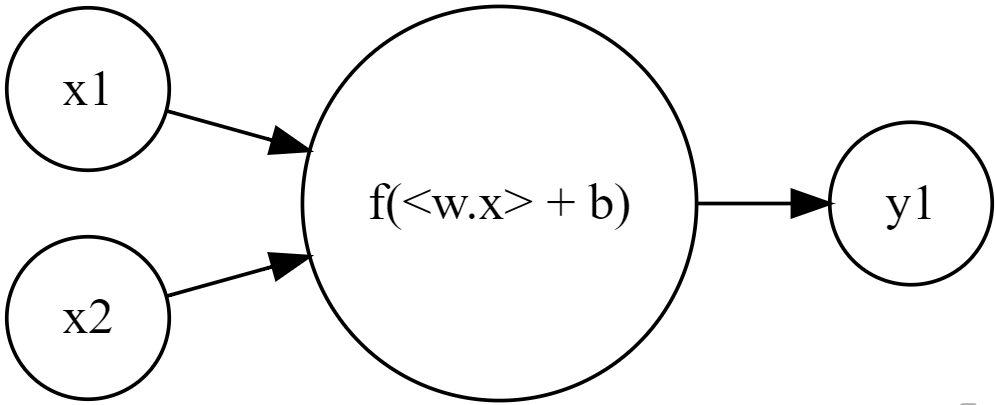
\includegraphics[width=8cm]{figuras/neuronio}
\caption{Rede neural mais simples ainda, apenas um neurônio oculto.}
\label{fig:neuronio}
\end{figure}

Esta rede possui $2$ neurônios na camada de entrada, que são os números reais $A$ e $B$, $1$ neurônio na camada oculta, no qual está a sua função de ativação $f(Ax + By)$, e $1$ neurônio na camada de saída, que neste caso é um número real $C$. Pode-se notar a semelhança dessa rede neural artificial com a sua inspiração biológica com a ajuda da figura~\ref{fig:neuron_model}. 

\begin{figure}[htb]
\centering
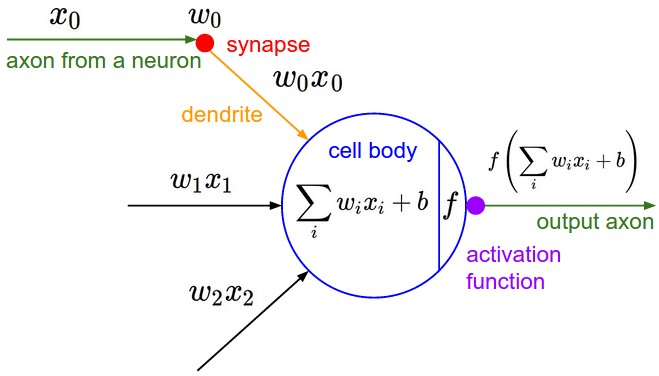
\includegraphics[width=8cm]{figuras/neuron_model}
\caption{Representação de um neurônio artificial.\footnote{Extraído de \url{https://cs231n.github.io/neural-networks-1/}}}
\label{fig:neuron_model}
\end{figure}

Temos os sinais de entrada (como o $x_0$) vindos como viriam os sinais dos axônios de outros neurônios. Eles entram pela camada de entrada da rede, ou dentritos do neurônio. A camada oculta processa as entradas com os pesos, definindo o sinal através de sua função de ativação, similar ao funcionamento do núcleo do neurônio que ativa ou não o sinal recebido. Por fim o sinal é enviado à camada de saída, ou aos axônios do neurônio, concluíndo o processamento.

\section{Sistemas nebulosos}

Os sistemas nebulosos foram criados a partir da teoria dos conjuntos nebulosos criada por L.A. Zadeh \citep{fuzzy_1}. Os conjuntos nebulosos diferem dos conjuntos clássicos na forma em que avaliamos se os elementos pertencem aos conjuntos ou não. 

Num conjunto clássico um elemento pertence a ele ou não, não há meio termo. Já nos conjuntos nebulosos existe uma função associando o grau com que um elemento pertence ao conjunto, a função assume $0$ se não pertence, ou seja, uma exclusão completa, e assume $1$ se pertence completamente, mas também assume qualquer valor real dentro deste intervalo. Esta é a chamada função de pertinência, de forma que a frase ``o elemento $x$ percente mais ao conjunto $A$ do que o elemento $y$'', por exemplo, é a representação verbal da expressão matemática $f(x) > f(y)$ se usarmos a definição de ordem dos números reais e da notação $f(.)$ para a função de pertinência.

Os sistemas nebulosos podem ser usados para modelar situações do mundo real que não podem ser muito bem representadas pelos conjuntos clássicos com seus limites muito bem definidos, mas melhor representadas pelos conjuntos nebulosos. Um exemplo ilustrativo é o do conceito de \emph{perto}.

Usar imagens e gráficos para mostrar esse exemplo aqui...

A partir disto, conforme descrito por L. Wang \citep{fuzzy_2}, os sistemas nebulosos são aproximadores universais. Isto significa que podem aproximar quaisquer funções numa grande variedade de de problemas. Neste artigo é demonstrado que com uma função de pertinência gaussiana é possível usar sistemas nebulosos para aproximar qualquer função real contínua definida num conjunto compacto.